\chapter{Dokumentation for brugergrænseflade}

\section{Indleding}

For at en bruger kan interagere med WinePrep skal der være en brugergrænseflade. Brugergrænsefladen skal give brugeren mulighed for at kunne benytte WinePreps funktioner. Der skal være mulighed for at brugeren kan benytte sig af muligheden ”Åben nu” som åbner vinen straks efter at kommandoen er givet. Yderligere skal der være mulighed for at brugeren kan planlægge åbningen af vinen således at man kan bestemme et tidspunkt på åbning af vinen. På brugergrænsefladen skal det også være muligt at kunne tilgå WineBook, WhíchWine, Indstillinger og Aktuel info. Under Aktuel info skal der fremgå hvor lang tid der er tilbage til åbning af vinen. Der er yderligere blevet gjort nogle overvejelser over designet på brugergrænsefladen. Nogle af disse overejelser vil blive præsenteret her.

\section{Design og implementering}
\subsection{Skitsering af brugergrænseflade}

Da touch-mekanismen på Devkit8000 ikke er helt optimal er det blevet besluttet at der skal benyttes store knapper således det ikke bliver svært at vælge de muligheder en bruger beslutter sig for at vælge. Den føste skitse for brugergrænsefladen så således ud:

\begin{figure}[H]
	\centering
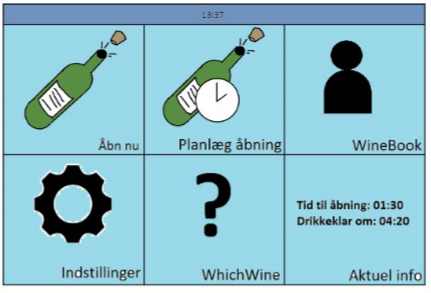
\includegraphics{Billeder/skitse}
\caption{Første skitse af brugergrænsefladen}
\end{figure}

\subsection*{Første udgave af brugergrænseflade}
På første udgave af produktet blev det dog besluttet at der ikke skal være nogen grafik på brugergrænsefladen. Yderligere blev det besluttet at det kun er funktionen Åbn nu der skal implementeres da det er denne funktion der danner grundlaget for funktionaliteten af produktet. Derfor blev Real Time Clocken  (RTC) heller ikke implementeret, og derfor kunne tiden heller ikke visen, hverken klokkeslættet eller på Aktuel info.
Et foreløbigt design på brugergrænsefladen ser således ud:

\begin{figure}[H]
	\centering
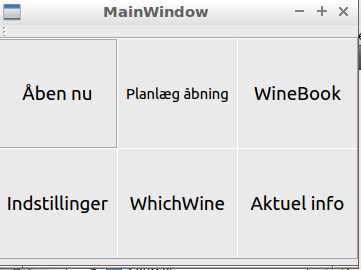
\includegraphics{Billeder/real_skitse}
\caption{Første skitse af brugergrænsefladen}
\end{figure}

Her kan det ses at der ikke er blevet sat fokus på design og grafik. Når der trykkes på knappen åben nu, vil programmet sende en kommando til PSOC ved hjælp af SPI om at flasken skal registreres. Dog bruges kun kommandoerne fread og fwrite til at skrive og læse fra en character device driver. Denne kode ses her:

\begin{figure}[H]
	\centering
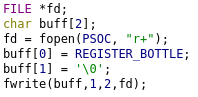
\includegraphics{Billeder/write}
\caption{Eksempel på brug af fwrite funktionen}
\end{figure}

For at få svar på om hvorvidt en flaske er registreret eller ej skal der læses via character device driveren. Dette gøres med funktionen fwrite(). Fwrite() ses brugt i følgende eksempel hvor der skal læses om flasken er blevet registreret:

\begin{figure}[H]
	\centering
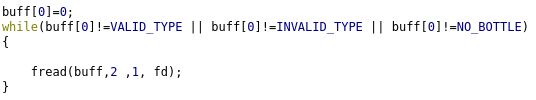
\includegraphics{Billeder/read}
\caption{Eksempel på brug af fread funktionen}
\end{figure}

Først nulstilles bufferen som skal indeholde kommandoen, og derefter læses der i en whilelykke. Når fread() læser VALID{\_}TYPE, INVALID{\_}TYPE eller NO{\_}BOTTLE vil whilelykken brydes og den læste kommando vil indsættes buff’s første plads. Når værdien indsættes i buff gennemgåes en switch-case hvor der alt efter hvilken værdi der er blevet læst ind i buff reageres på forskellige måder. Et eksempel ses her:

\begin{figure}[H]
	\centering
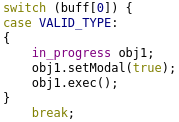
\includegraphics{Billeder/switch}
\caption{Eksempel på brug af switch-case efter at have læst fra PSoC}
\end{figure}

Denne kode vil resultere i at der kommer et vindue op hvor der står ”Vinen åbnes. Vent venligst…”. Man vil få muligheden for at trykke ok for at få vinduet til at forsvinde igen. 
Efter dette vil vinåbningen enten lykkedes eller fejle. Devkit8000 vil derefter få besked om åbningen er lykkedes eller om den er fejlet. Der vil endnu engang benyttes en switch case til at bestemme hvilken besked brugeren får frem på brugergrænsefladen.
Selve klikfunktionen på de forskellige knapper er implementeret ved at højreklikke på de forskellige knapper og trykke på goto. Herefter vil der dukke en ny menu op. Her vælges clicked(). Her vil man få mulighed for at bestemme hvilken funktion knappen skal have når den trykkes. Et eksempel ses her:

\begin{figure}[H]
	\centering
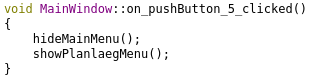
\includegraphics{Billeder/pushButton}
\caption{Implementering af trykknappen Planlæg åbning}
\end{figure}

Dette er implementeringen for planlæg åbning knappen. Det der sker når man trykker på knappen er, som det fremgår på kodeeksemplet, at hovedmenuen skjules, og at Planlægningsmenuen vises. 
Måden hvorpå menuskiftsfunktionen er blevet implementeret er ved brug af show og hide funktionerne i QT. Dette kan ses i følgende eksempel hvor tilbageknappen skjuler alle knapper på den nuværrende menu, for derefter at vise alle knapper på hovedmenuen:

\begin{figure}[H]
	\centering
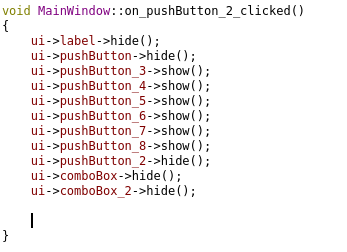
\includegraphics{Billeder/tilbageKnap}
\caption{Skift af menu med tryk på tilbageknappen}
\end{figure}

\section*{Test}

Som tidligere beskrevet er der i første udgave kun implementeret Åbn nu funktionen. Derfor er det kun denne funktion der kan testes. Dog kan navigationen på de forskellige menuer på brugergrænsefladen også testes. Menuerne WineBook, WhichWine, Indstillinger og Aktuel info er ikke blevet implementeret i denne udgave, og derfor vil test af disse menuer ikke fremgå i denne test.

Read og write funktionerne testes ved at tilkoble en PSoC til Devkit8000 og forsøge at skrive og læse til og fra den. Der er blevet konstrueret nogle meget simple forsøg, hvor funktionerne fread og fwrite bruges. Forsøget er konstrueret således at en led på PSoC'en lyser hver gang der læses fra den. Yderligere vil det der læses fra PSoC'en skrives til en fil på devkitted. Forsøget hvor der læses fra Devkit8000 er vedhæftet som en fil i bilaget, hvor man kan se at led'en på PSoC'en tænder og slukker hver gang der trykkes på Åbn nu på brugergrænsefladen. Koden der er brugt til at teste forbindelsen med er følgende:

\begin{figure}[H]
	\centering
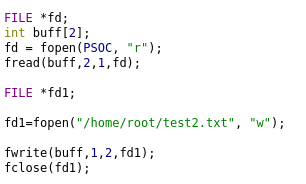
\includegraphics{Billeder/testKode}
\caption{Kode til test af forbindelse}
\end{figure}

Denne kode tester blot fread og fwrite funktionerne. PSoC'en er programmeret således at dens LED lyser hver gang der bliver læst fra den. Yderligere gemmer koden det den læser i en tekstfil på devkitted.

Når man trykker på knappen Planlæg åbning dukker følgende menu op:

\begin{figure}[H]
	\centering
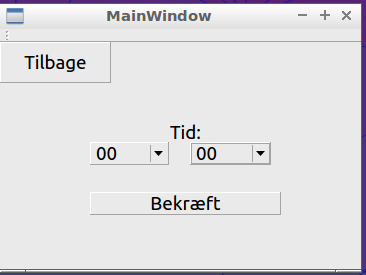
\includegraphics{Billeder/paMin}
\caption{Menu til planlæg åbning med scrolldown menu åben for timer}
\end{figure}

For minutter ser det således ud:

\begin{figure}[H]
	\centering
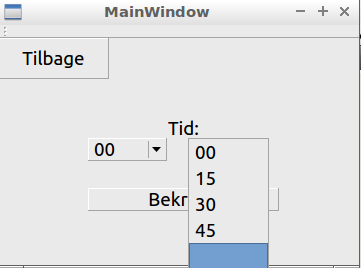
\includegraphics{Billeder/paMinutter}
\caption{Menu til planlæg åbning med scrolldown menu åben for timer}
\end{figure}
\section*{Resultater}

Da hele produktet ikke er fuldt udviklet er det ikke muligt at fremvise nogle resultater. Man kan se på videoen at vi kommer til at tænde og slukke for dioden ved hjælp af brugergrænsefladen på devkittet. Videoen kan ses i bilaget.

\section*{Konklusion}

Alle test gik som forventet, da dioden på PSoC'en kom til at tænde ved læsning som forventet. Yderligere er designet for brugergrænsefladen, og navigationen i den blevet som forventet. Dog blev designet ikke implementeret, da dette vil gøres i en senere itteration.